\documentclass[twoside, type=msc,colorback,accentcolor=tud1b, 11pt, numbersubsubsec]{tudthesis}
\usepackage[german]{babel}
\usepackage{mathtools}
\usepackage{graphicx}
\usepackage{hyperref}
\usepackage{wrapfig}
\usepackage{enumitem}
\usepackage{framed}
\usepackage{mdframed}
\usepackage{courier}
\usepackage{amsmath}
\usepackage{todonotes}
\usepackage{booktabs}

\mdfsetup{nobreak=true}
\mdtheorem{definition}{Definition}
\mdtheorem{formula}{Formula}

% todonotes setup
\newcommand{\addcitation}[1]{\todo[color=yellow,inline]{Missing citation: #1}}
\newcommand{\outline}[1]{\todo[color=pink,inline]{Outline: #1}}

\usepackage{float}
% Figure caption
\usepackage{caption}
\captionsetup[figure]{name=Figure}
\captionsetup[table]{name=Table}
\usepackage{subcaption}

% Paragraph style
\setlength{\parindent}{0cm}
\setlength{\parskip}{1em}

\DeclareMathSizes{11}{14}{9}{9}
\linespread{1.3}

\newcommand{\getmydate}{%
  \ifcase\month%
  \or Januar\or Februar\or M\"arz%
  \or April\or Mai\or Juni\or Juli%
  \or August\or September\or Oktober%
  \or November\or Dezember%
  \fi\ \number\year%
}

\parskip=2mm

\begin{document}
\thesistitle{Using Deep Learning Methods to Predict Tweet Engagement Metrics}{}

\author{Felix Peters}
\birthplace{Bad Soden am Taunus}

\department{Fachbereich Rechts- und Wirtschaftswissenschaften}
\group{Wirtschaftsinformatik}
\referee{Prof. Dr. Peter Buxmann}{Prof. Dr. Alexander Benlian}

% Start of text output
\makethesistitle

% TODO: Change
\affidavit[24. April 2018]{Felix Peters}

\section*{Abstract}

This is my abstract.


\renewcommand{\contentsname}{Table of contents}
\tableofcontents

%\renewcommand{\listfigurename}{List of figures}
%\listoffigures
%
%\renewcommand{\listtablename}{List of tables}
%\listoftables

\section{Introduction}
\label{ch:introduction}

Here comes a beautiful introduction.

\section{Background}
\label{ch:background}

This chapter serves to explain the foundations of natural language processing (NLP), especially the subpart of language modeling, needed to understand the problem and methodology used in this thesis. The two main building blocks of this thesis are the examination of a state-of-the-art language model (LM) and its ability to generate high quality, human-like text on the one hand and methods to distinguish such generations from human written text on the other hand. In order to understand the problem and methodology used in this thesis, this chapter explains the foundations of NLP (ch.~\ref{sec:history_of_language_modeling}), especially the subpart of language modeling, and the foundations of deep learning (ch.~\ref{sec:deep_learning_in_machine_learning}) especially under the aspect of sequence classification.

\subsection{Deep learning in machine learning}
\label{sec:deep_learning_in_machine_learning}

This section aims to firstly embed the field of deep learning, which is the current driver of the latest progress in the field of \textbf{natural language processing (NLP)}\footcite{Deng2018}, into machine learning. The first subsection (ch.~\ref{sub:definition}) will define machine learning and especially deep learning and will go over the most common terminology found in these fields. Afterwards (ch.~\ref{sub:neural_networks}), neural networks as the key concept for deep learning will be introduced. Later on (ch.~\ref{sub:recent_developments}) recent developments will be presented and the chapter will be concluded by giving an overview of practical applications of deep learning (ch.~\ref{sub:practical_applications}). The notation used throughout this chapter mostly follows the one used by Bishop~\footcite{bishop2006pattern} in his book “Pattern Recognition and Machine Learning“. Here scalar values are noted as lowercase letters (e.g. $ x $), vectors as bold lowercase letters (e.g. $ \pmb{b} $) and matrices as bold uppercase letters (e.g. $ \pmb{W} $).

\subsubsection{Definition}
\label{sub:definition}

\begin{quote}
For thousands of years, we have tried to understand how we think; that is, how a mere handful of matter can perceive, understand, predict, and manipulate a world far larger and more complicated than itself. The field of artificial intelligence, or AI, goes further still: it attempts not just to understand but also to build intelligent entities.
\end{quote}

This is the quote used by Stuart Russel and Peter Norvig~\footcite{russell2016artificial} to introduce the field of \gls{ai} in their book “Artificial Intelligence: A modern approach“.

In order to give a clear overview of the topics of \gls{ml} and especially deep learning it is important to clearly separate terms that are commonly used interchangeably. While many different definitions for \gls{ai} can be found, it generally refers to the borader concept of creating general purpose machines that can perform tasks that are characteristic of human intelligence. To achieve this, machines need to detect patterns in data they are fed and to build up knowledge from these patterns.

The fundamental goal of \gls{ml} is to develop a \textit{machine} or an \textit{algorithm} that \textit{learns} to perform a \textit{task} from \textit{past experience}. More abstractly, our goal is to learn a mapping from input to output
\begin{equation}
	f : I \rightarrow O
\end{equation}
which can also be written as
\begin{equation}
	y = f(x ; \theta)
\end{equation}
where $ x \in I $ denotes the input, $ y \in O $ denotes the output and $ \theta \in \Theta $ denotes the parameters of the model.

To have a well-functioning model, different steps have to be completed. First of all, we need proper inputs (and outputs) in the form of data entries suited for the problem. These data entries are then typically split into two subsets called the \textit{training} data and the \textit{test} data. Then, the training data is used to tune the model parameters, or \textit{weights}, to minimize the difference between the model prediction and the desired output. With the test data, one can evaluate how good the model is at performing the given task by comparing the prediction with the “true“ or the desired result. Hereby, \gls{ml} models are divided into different categories depending on either their type of problem and the format of their training (and test) data.

\paragraph*{Problem type}
The first distinction can be made along the value range of the output variable. If the model learns a mapping into a discrete space (e.g. \{1, 2, ..., 10\}), then we are talking about a \textbf{classification} problem. The perhaps most famous example for this task is the MNIST handwritten digit classification~\footnote{\url{http://yann.lecun.com/exdb/mnist/}}, where a model learns to recognize handwritten digits provided in the form of images. Another example could be the recognition of music genres given the audio input files. If, however, the model learns a mapping into a continuous space (e.g. $ O = {\rm I\!R} $) , then we are talking about a \textbf{regression} problem. For this problem, the prediction of the value of a house given certain features such as the property square meters or the location in the city (e.g. “good“ or “bad“) can be listed. \textbf{Density estimation} is the task of being confronted with data points for which one does not know the underlying distribution. Taking a look at the locations of a dart disk that a dart that was thrown several times landed on might show us that we are dealing with an inverse two dimensional gaussian distribution. The last problem type that will be listed is the one of \textbf{clustering}: Here, one is faced with data points and shall determine (the amount of) class types that best encapsualte groups within the data points. One such example could be a streaming provider that wants to determine what kinds of viewer groups it has to perform further marketing and personalization strategies. Other \gls{ml} task definitions and examples can be found in subject specific literature or internet.

\paragraph*{Data format}
In a \textbf{supervised learning} environment, both the input and the output data points are made available to the model. This allows us to compute a distance function between output and desired result, also called cost function (ch. 3.3.3). Using this cost function as a performance measure, the model is able to give more accurate predictions over time by optimizing the cost function at each step (see above classification and regression examples). In an \textbf{unsupervised learning} environment, we only get the raw data entries without the desired output, or \textit{labels}. As we therefore have no metric for calculating the distance between prediction and label we can not perform classification or regression tasks. Problems that can be tackled with unsupervised learning are clustering and density estimation. If the data set is split into data points with labels and data points without labels we speak of \textbf{unsupervised learning}. The motivation for semi-supervised learning is that readily available and unlabeled data can be used to improve supervised learned models when labeled data are scarce or expensive. It can also seen as a quantitive tool to understand human category learning, where most of the input is self-evidently unlabeled~\footcite{6813505}. The last \gls{ml} paradigm is called \textbf{\gls{rl}}. In this setting, “learning is learning what to do — how to map situations to actions — so as to maximize a numerical reward signal. The learner is not told which actions to take, but instead must discover which actions yield the most reward by trying them“~\footcite{10.5555/551283}. Even though the reward policy - that is, the definition of good and bad results - is set by the programmer, the model is given no heuristics or concepts for solving the problem. It is up to the model to figure out how to perform the task to maximize the reward , starting from totally random trials and finishing with sophisticated tactics. An example would be the inverted pendulum problem: This tasks consists of balancing a pendulum that has its center of mass above its pivot point on a moving platform - it is unstable and will fall over without additional help. This “help“ consists of moving the platform either forward and backward (or left and right).

% \begin{figure}
% 	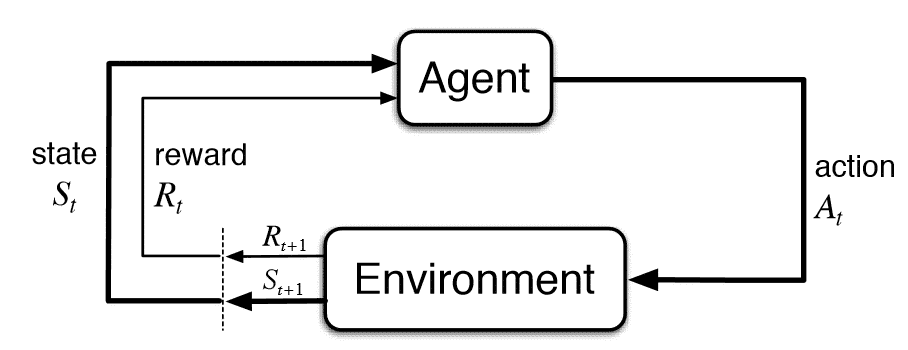
\includegraphics[height=4cm]{img/reinforcement_learning_cycle}
% 	\caption{Reinforcement learning cycle}
% 	\label{fig:reinforcement_learning_cycle}
% \end{figure}


\subsubsection{Neural networks}
\label{sub:neural_networks}

The origins of the term \textit{\gls{nn}} lie in the attempt to find mathematical representations of information processing in biological systems such as the human brain where the sheets of tissue may be understood as vectors of neurons. While assuming biological realism in pattern recognition is impractical and imposes too many unnecessary constraints, \gls{nn}s have proven to be capable of solving complex problems. The main reason for this is being able to get rid of the task of feature selection. Before the rise of \gls{nn}s, scientists and researchers had to complete the laborious task of coming up with good features to solve learning problems. Their structure enables the learning of useful representations of the input data by creating complex data representations through the combination of simpler ones. The most simple and also most successful model of this type is known as the (three layered) \textbf{\gls{mlp}} (in the following simply denoted as \gls{nn}), which will now shortly be presented. Later on (subsection~\ref{sub:neural_language_models}), more complex neural network architectures will be presented especially under the aspect of their aptitude for \gls{nlp}tasks.

A typical linear model for regression or classification is based on linear combinations of fixed nonlinear basis functions $ \phi_j (\pmb{x}) $ and takes on the form
\begin{equation}
	\label{eq:lin_comb_of_nonlinear_basis_func}
	y(\pmb{x}, \pmb{w}) = f \left( \sum_{j=1}^{M} w_j \phi_j (\pmb{x}) \right)
\end{equation}
where $ f(\cdot) $ is a nonlinear activation function. How \gls{nn}s extend this model is by making the basis functions $ \phi_j(\pmb{x}) $ depend on the parameters and then allow these parameters to be adjusted, along with the coefficients $  \{w_j\} $ during training. This gives us a basic \gls{nn} that can be described as a series of functional transformations. First, $ M $ linear combinations of the input variables $ x_1, \dots, x_D $ in the form
\begin{equation}
	a_j = \sum_{i=1}^{D} w_{ji}^{(1)} x_i + w_{j0}^{(1)}
\end{equation}
need to be constructed where $ j = 1, \dots, M $ with $ M $ being the number of hidden neurons, $ D $ denotes the input dimension and the superscript $ (1) $ indicates that the corresponding parameters are in the first `layer' of the network. The model parameters $ w_{ji}^{(1)} $ are called \textit{weights} and the parameters $ w_{j0} $ are called \textit{biases}. The term $ a_j $ is known as an \textit{activation}. Each activation is then transformed using a differentiable, nonlinear \textit{activation function} $ h (\cdot) $ to give the final output of a neuron:
\begin{equation}
	z_j = h(a_j)
\end{equation}
These quantities are called the \textit{hidden units}. The introduction of non-linearity into the network through these activation functions is a key factor in the success of \gls{nn}s as only using linear activation functions would allow for a creation of an equivalent network without hidden units. This is due to the fact that the composition of successive linear transformations is itself a linear transformation~\footnote{\url{http://www.math.lsa.umich.edu/~kesmith/217worksheet2-3ALT1.pdf}}. As for the implementation of these activation functions there exist different variants that will be listed and explained in the paragraph '\nameref{par:activation_function}'. Following equation~\ref{eq:lin_comb_of_nonlinear_basis_func}, these values are again linearly combined to give \textit{output unit activations}
\begin{equation}
	\label{eq:output_unit_activation}
	a_k = \sum_{j=1}^{M} w_{kj}^{(2)} z_j + w_{k0}^{(2)}
\end{equation}
where $ k = 1, \dots, K $ and $ K $ is the total number of outputs. Equation~\ref{eq:output_unit_activation} represents the second layer of the network. Finally, the output unit activations are transformed using an appropriate activation function to give a set of network ouputs $ y_k $. \\
Now, we can combine these various stages to give the overall network function that takes the form
\begin{equation}
	y_k(\pmb{x}, \pmb{w}) = f \left( \sum_{j=1}^{M} w_{kj}^{(2)} h \left( \frac{1}{2} \right) + w_{k0}^{(2)} \right)
\end{equation}
Thus the neural network model is simply a nonlinear function from a set of input variables $ \{x_i\} $ to a set of output variables $ \{y_k\} $ controlled by a vector $ w $ of adjustable parameters.

Figure~\ref{fig:neural_network_architecture} shows the main components of the \gls{mlp}. The input, hidden, and output variables, or units, are represented by nodes, and the weight parameters, or simply \textit{weights}, are represented by links between the nodes. Additionally, bias parameters, or simply \textit{biases}, are denoted by links coming from additional input and hidden variables $ x_0 $ and $ z_0 $. The arrows demonstrate the direction of information flow through the network during forward propagation.
\begin{figure}
	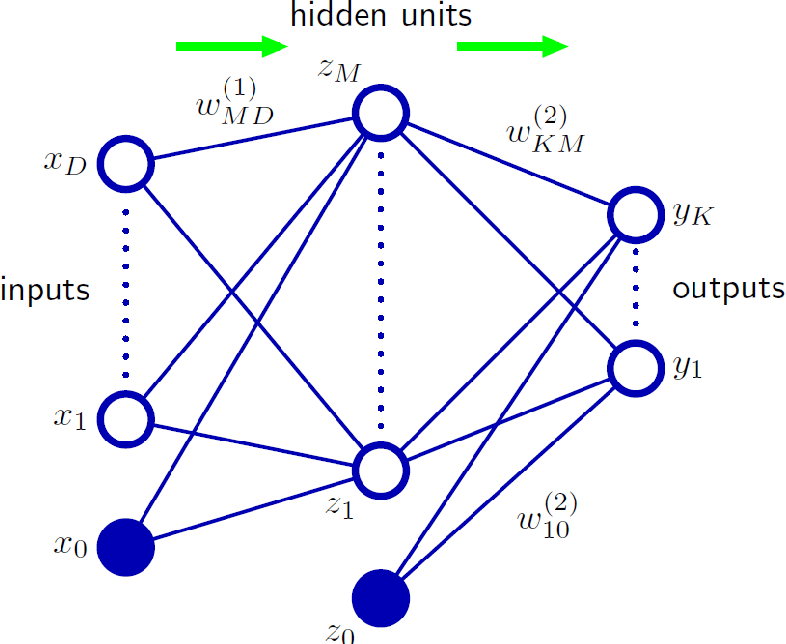
\includegraphics[height=8cm]{img/neural_network_structure}
	\caption{Neural network architecture}
	\label{fig:neural_network_architecture}
\end{figure}

\paragraph{Training process}\label{par:training_process}
The actual tuning of the network's weights are not determined exactly but are usually initialized randomly and iteratively optimized using training data via \textbf{forward propagation}. As this falls into the category of supervised learning, the desired outputs for the training inputs are known and thus a \textbf{cost} or \textbf{loss} function can be used to assess the discrepancy between prediction and ground truth. The calculated error can be used to determine the necessary updates on the weights to improve the predictions in a process called \textbf{backpropagation}. These steps will now be explained individually and in detail.

\paragraph{Activation function}\label{par:activation_function}
In analogy to our biological neurons, artificial neurons can fire a signal depending on the provided input to communicate with the following neurons (or in biology: with the neurotransmitters through electrical impulses). The decision whether a neuron fires or not lies with the activation function. After a single neuron calculates a weighted sum of its input and adds a bias to it, the value of the calculation can be anything from $ -\infty $ to $ +\infty $. As the neuron does not know the bounds of the value it uses an activation function to determine whether it should fire a signal or not.
The easiest option would be to just implement a threshold that fires if $ y > 0 $ and else does not. This, however, poses a problem when dealing with for example multi-classification. In a setting where we have 10 classes and have 2 neurons firing we can not safely say which class the model is more confident on. It would be more helpful to have instead an output of `60\%' or `90\%' activation. A linear function would also not be suited, because of the aforementioned possibility that many linear layers can be replaced by a single layer. That is why most \gls{nn}s nowadays use well-known and established activation functions in their architectures. One of the oldest but still widely used activations is the \textbf{sigmoid function} (in the form of the logistic function)
\begin{equation}
	S(x) = \frac{1}{1+e^{-x}} = \frac {e^{x}}{e^{x}+1}
\end{equation}
The sigmoid function is nonlinear and has no binary activations. Furthermore, it has a smooth gradient which means that the output does not jump in big value ranges. Sigmoids are especially suited for classification tasks, as they tend to bring activations to either `side' of the curve allowing for clear distinctions on prediction. Nonetheless, sigmoids also have a downside: Towards the edges of the domain, the slope on the $ y $-values increases (decreases) less and less which in turn also makes the gradient smaller. This poses a problem as the gradient amongst other things dictates the learning progress of the neural network - and a non-existent gradient also means that there is no learning progress (this problem is typically referred to as \textit{vanishing gradient}). Another frequently mentioned activation function is the \textbf{hyperbolic tangent}
\begin{equation}
	\tanh(x) = \frac{\sinh(x)}{\cosh(x)} = \frac{e^{x}-e^{-x}}{e^{x}+e^{-x}} = \frac{e^{2x}-1}{e^{2x}+1}
\end{equation}
which is basically a scaled sigmoid function. The $ tanh $ function was introduced in order to provide a stronger gradient than sigmoid (for steeper derivatives). Whether sigmoid or tanh activation functions should be chosen depends on the nature of the problem. The sigmoid activation function saturates at zero and one while tanh saturates at plus and minus one. So if the activity in the network during training is close to zero then the gradient for the sigmoid activation function may go to zero. However, the activation function that has had by far the most impact in the world of \gls{ml} and especially deep learning is the \textbf{\gls{relu}}
\begin{equation}
	f(x) = x^{+} = \max(0,x)
\end{equation}
simply because of its non-saturation gradient, which greatly accelerates the convergence of stochastic gradient descent compared to the other two functions~\footcite{10.1145/3065386}. Another useful property of the \gls{relu} function is that it does not need any expensive operations (e.g. exponentials) to be computed, but can simply be implemented by thresholding a matrix of activations at zero.
\begin{figure}
	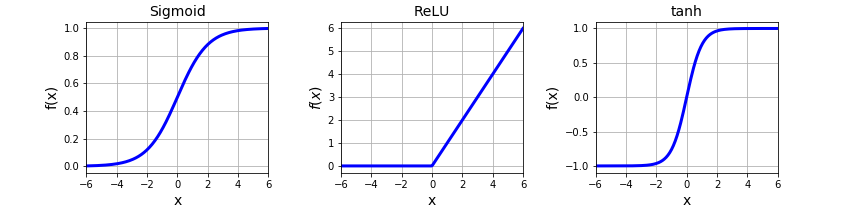
\includegraphics[height=4cm]{img/activation_functions}
	\caption{Different activation functions}
	\label{fig:different_activation_functions}
\end{figure}

\paragraph{Cost function}\label{par:cost_function}
For a neural network to know how and when to update its parameters it needs to know what the underlying optimization problem is that it is facing. This is posed by the so-called \textit{cost function}, or \textit{loss function}, which compares the prediction of the model with the desired value and returns a metric of distance. The gradient at the given input values determines the updates that the neural network will perform on its weights and biases. In the following, two of the most prominent loss functions will be presented and explained. Here, $ y $ denotes the true solution and $ \widetilde{y} $ denotes the prediction as a function $ h $ with parameters $ \theta $ of the input $ x $ of the model. The general equation of a cost function represents the sum of the errors multiplied across the whole batch:
\begin{equation}
	J(\theta) = \frac{1}{\alpha} \sum_{i=1}^{n} \text{C} (h_{\theta} (y^{(i)}), \widetilde{y}^{(i)})
\end{equation}
A simple implementation of the cost function is the \textbf{\gls{mse}} loss, which has analogies to many fields such as mechanical engineering~\footnote{\url{https://projecteuclid.org/download/pdf_1/euclid.bbms/1203692451}}. Here, the square of the difference between prediction and truth is squared, summed up and then divided by the length of the batch.
\begin{equation}
	\frac{1}{N} \sum_{i=1}^{N} \left( y_i - \widetilde{y_i} \right)^2
\end{equation}
One of the standard functions when it comes to classification is the cross-entropy loss function that calculates on step $ t $ the cross-entropy between predicted probability distribution $ \hat{y}^{(t)} $, and the truth $ y^{(t)} $
\begin{equation}
	J^{(t)}(\theta) = \text{CE}(\pmb{y}^{(t)}, \hat{\pmb{y}}^{(t)}) = - \sum_{w \in V} \pmb{y}_w^{(t)} \ \text{log} \ \hat{\pmb{y}}_w^{(t)} = - \text{log} \ \hat{\pmb{y}}_{\pmb{x}_{t+1}}^{(t)}
\end{equation}
Cross entropy relies on probabilities and not just boolean values for class membership, therefore, it allows more precise performance evaluation. Abstractly, cross entropy between two probability distributions can be interpreted as the expected message-length per datum when a wrong distribution $ q $ is assumed while the data actually follows a distribution $ p $.

\paragraph{Backpropagation}\label{par:backprop}
The process of calculating the activations at each hidden layer and the output layers as well as the resulting loss function is known as \textbf{forward propagation}. Now, to actually update the parameters of the neural network the \textit{contribution} of each parameter to the loss (gradient) needs to be computed and each parameter needs to be updated with gradient descent - this process is called \textbf{backpropagation}. The concept of gradient descent can be illustrated in a two-dimensional setting by plotting the `landscape' of the loss function which one is trying to minimize - here the initial value can be seen as the start position of a `ball' that then starts to roll down until it reaches the bottom, or mathematically: the local minimum (figure~\ref{fig:gradient_descent}). The idea of backpropagation was introduced in the 1970s by Finnish master student Seppo Linnainmaa~\footcite{linnainmaa1970representation}. Here, instead of naively calculating the gradient of each layer separately the partial computations of the gradient for each layer are reused in the computation of the gradient for the previous layer. The backpropagation algorithm is dependent on the following 5 equations:

The partial derivatives of the cost function are calculated by
\begin{equation}
	\label{eq:backprop_one}
	\frac{\delta J}{\delta w_{ij}^{k}} = \delta_j^k o_i^{k-1}
\end{equation}
where for each $ \delta_j^k $ is calculated on the final layer's loss term
\begin{equation}
	\label{eq:backprop_two}
	\delta_1^m = g'_o (a_1^m)(\hat{y}_d - y_d)
\end{equation}
and on the hidden layers' loss terms
\begin{equation}
	\label{eq:backprop_three}
	\delta_j^k = g'(a_j^k) \sum_{l=1}^{r^{k+1}} w_{jl}^{k+1} \delta_l^{k+1}
\end{equation}
Combination of the partial derivatives for each input-output pair are takes places like so
\begin{equation}
	\label{eq:backprop_four}
	\frac{\delta J(X, \theta)}{\delta w_{ij}^k} = \frac{1}{N} \sum_{d=1}^{N} \frac{\delta}{\delta w_{ij}^{k}} \left( \frac{1}{2} (\pmb{\hat{y}_d} - \pmb{y_d})^2 \right) = \frac{1}{N} \sum_{d=1}^{N} \frac{\delta J_d}{\delta w_{ij}^k}
\end{equation}
As for updating the weights, one uses
\begin{equation}
	\label{eq:backprop_five}
	\Delta w_{ij}^{k} = - \alpha \frac{\delta J(X, \theta)}{\delta w_{ij}^{k}}
\end{equation}
In the following the simplest form of backpropagation with simple \textit{gradient descent} will be presented.
\begin{enumerate}
	\item Firstly, the forward propagation for each input-output pair $ \pmb{x_d}, \pmb{y_d} $ has to be computed. The results $ \pmb{\hat{y}_d} $, $ \pmb{a_j^k} $ and $ o_j^k $ for each node $ j $ are then stored in layer $ k $ by proceeding from input layer $ 0 $ to the output layer $ m $.
	\item Secondly, the backward phase for each input-output pair $ \pmb{x_d}, \pmb{y_d} $ is calculated and the results $ \frac{\partial J_d}{\partial w_{ij}^{k}} $ for each weight $ w_{ij}^{k} $ connecting node $ i $ in layer $ k - 1 $ to node $ j $ in the next layer are stored starting now on the last layer $ m $ and continuing until layer $ 1 $. This step can be further split up into 3 sub-steps:
	\begin{enumerate}
		\item The term $ \delta_1^m $ is calculated by using equation~\ref{eq:backprop_two}.
		\item The calculated loss terms for the hidden layers $ \delta_j^k $ are backpropagated starting on layer $ k = m - 1 $ through repetitive usage of equation~\ref{eq:backprop_three}.
		\item Now the partial derivatives of individual loss $ J_d $ \gls{wrt} $ w_{ij}^k $ can be evaluated by using equation~\ref{eq:backprop_one}.
	\end{enumerate}
	\item Now, the entirety of the gradient $ \frac{\delta J(X, \theta)}{\delta w_{ij}^k} $ over the entire set of input-output pairs can be calculated by combining the individual input-output pair gradients in equation~\ref{eq:backprop_four}.
	\item The \textbf{learning rate} $ \alpha $ is used in the final formula to update the weights of the network by subtracting the total gradient $ \frac{\delta J(X, \theta)}{\delta w_{ij}^k} $ multiplied by $ \alpha $ (equation~\ref{eq:backprop_five}).
\end{enumerate}
\bigskip

\begin{figure}
	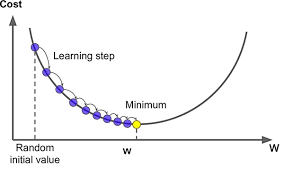
\includegraphics[height=4cm]{img/gradient_descent}
	\caption{Gradient descent on a convex quadratic function}
	\label{fig:gradient_descent}
\end{figure}

There are different variations of the gradient descent optimization, namely batch, stochastic and mini-batch, which will shortly be presented. Each variant differs in how much data is used to compute the gradient of the loss function - which one is best suited depends on the problem. These variations fundamentally are a trade-off between speed and accuracy. \textbf{Batch gradient descent} utilizes the whole dataset, computing the loss of each data point and averaging over the entire set. This takes up a lot of computation, therefore batch gradient descent is considered to be slow. Also using each datapoint many times can cause the algorithm to overfit on the training data. Batch gradient descent works best for functions with very little local minima, as it can easily get stuck in one. In contrast, \textbf{\gls{sgd}} computes the loss and makes the update on a single sample rather than the entire set. This speeds up each gradient step linearly with the size of the data set. Due to noise in the data it can happen though, that the gradient step is performed in the opposite direction of the optimum. \gls{sgd} works best if the function has a lot of local minima since the noise performing the gradient descent on a single data point oftentimes moves the model out of local minimum to maybe a better one. \textbf{Mini-Batch} uses a random subset of the entire dataset and computes the gradient of the loss on that subset. This is a combination of the other two methods so it can reduce the problems they are facing. It takes way less computation performing one step while reducing the noisiness of \gls{sgd}. Choosing the mini-batch size depends on the problem. If possible it should be small enough to still avoid local minima, while being big enough to converge to the global minimum.



\subsubsection{Best practices and design choices}
\label{sub:best_practices_and_design_choices}

This subsection will list and describe important metrics, heuristics and design choices that are either fundamentally important for deep learning or that will be used throughout this work.

\paragraph{Optimization}
Here I talk about Adam and better gradient techniques such as gradient clipping, dropout(?) and residual connections.

\paragraph{Sampling strategies}
Write about beam search, top-k and nucleus sampling.

\paragraph{Regularization and normalization}
Write about dropout and label smoothing as well as batch and layer normalization

\paragraph{Perplexity}
Write about perplexity.

\paragraph{Transfer learning and fine-tuning}
Currently, for many machine learning tasks, more computing power seems to lead predictably to better performance, and is often complementary to algorithmic advances. This is a statement that has never been so true as it is now. Consequently, training a current state-of-the-art model requires signficant hardware and data resources. While most available \gls{nlp} models ten years ago could be developed and trained with commercial laptops or servers, nowadays much specialized hardware in form of GPUs and TPUs is needed (although research for fast CPU algorithms is conducted as well~\footnote{\url{https://hothardware.com/news/researchers-slide-algorithm-cpu-ai-training-outperforms-gpu}}). One way to face this challenge and still achieve high performance results is through the field of sequential \textbf{transfer learning}, where tasks are learned successively. Transfer learning allows models to be trained for similar tasks or domains to increase their generalization capabilities. This can then lead to models achieving better results in areas outside of their initial specification. Sequential transfer learning comprises two phases: During the \textit{pretraining} phase, the model is trained to learn very general representations for a source domain. Afterwards, in the \textit{adaptation} phase, the model is specifically trained to perform well on a (usually more narrow) target domain. This adaptation, or fine-tuning, phase introduces a minimal set of task-specific parameters for subsequent tasks. In contrast to the transfer learning approach, classical models perform isolated learning of a single prediction model for a certain task - this is mainly suitable for well-defined, narrow tasks and requires training of the model from scratch. \\
Pretraining of \gls{lm}s has proven to be an effective method for improving many \gls{nlp} tasks~\footcite{DBLP:journals/corr/abs-1801-06146}. This shift also allows for an efficient and resource-saving adaptation to the target task while at the same time maintaining (or increasing) performance. Another advantage is that the development of \gls{nlp} systems is accelerated by more easily reusable and better-known systems.


\subsubsection{Practical applications}
\label{sub:practical_applications}

Here I write about practical applications.

\subsection{History of language modeling}
\label{sec:history_of_language_modeling}

Natural language processing (NLP) is “an area of research and application that explores how computers can be used to understand and manipulate natural language text or speech to do useful things”~\footcite{doi:10.1002/aris.1440370103}. The applications of NLP such as speech recognition, sentiment analysis, question answering and others are numerous~\footcite{DBLP:journals/corr/GattK17}. Moreover, these applications are already being heavily used by industry and consumers alike e.g. in the forms of digital voice assistants, sentiment analysis for recommender systems and browser search bars~\footcite{8012330,10.1145/3064663.3064672,GoogleSearch}. The subcomponent of NLP needed when it comes to tasks like machine translation, predictive typing or summarization that involve either generating text or estimating the probability of text is called language modeling. The following notation mostly follows the one from the CS224 Stanford Natural Language Processing with Deep Learning lecutre by Chris Manning~\footnote{\url{https://web.stanford.edu/class/cs224n/index.html}}. The following chapters will cover word representation (ch.~\ref{sub:word_representation}) as the foundation for language models, followed by a brief explanation of the basics of language models (ch.~\ref{sub:foundations_of_language_modeling}) and will end with the most common and most used language model types and architectures (ch.~\ref{sub:n_gram_models} - ch.~\ref{sub:neural_language_models}).

\subsubsection{Word representation}
\label{sub:word_representation}

The starting point for most NLP related tasks lies within the preprocessing of the textual input data. These must first be converted into a semantically meaningful numerical representation to allow for effective computation. The simplest way to represent a word numerically is by treating words as \textit{one-hot} vectors. Using this format, one word is encoded into an $ n $-dimensional vector of numbers where $ n $ is the vocabulary size and each entry takes on the value $ 0 $ except for the one that corresponds to the indexed word which takes on the value $ 1 $. This process generates very sparse feature vectors for each input word, which is no problem for simple classification tasks, but is unsuitable for larger problems as the dimension size increases for each word added to the vocabulary. Another issue of one-hot vectors is the fact that these representations hold no notion of similarity: If we take a look at the representations for the words “plane“ and “airplane“ we would get two vectors that are orthogonal, just as any two vectors in the whole vocabulary. This poses a problem as every word's similarity to other words is the same and we can not encapsulate the meaning of the word. Yoav Goldberg writes in his primer on neural networks for language processing that one-hot vectors should only be considered for problems where the model has only a small amount of input features, the inputs do not have to share model parameters and where there is a lot of data to learn from~\footcite{DBLP:journals/corr/Goldberg15c}.

Otherwise, the currently dominant approach in the field is to use word embeddings as feature vectors. Word embeddings follow the so called “distributional semantics“, which state that a word's meaning is given by the words that tend to occur in a similar context. This idea of context-dependent nature of meaning was first introduced by english linguist J.R. Firth~\footnote{\url{https://web.stanford.edu/class/linguist236/materials/ling236-handout-05-09-vsm.pdf}} with the famous quote:

\begin{quote}
  You shall know a word by the company it keeps.
\end{quote}

Following this idea we represent each word by a distribution of weights across many dimensions. Now, instead of having a one-to-one mapping between an element in the vector and a word, the representation of a word is spread across all of the entries in the vector, and each element in the vector contributes to the definition of many words. Having this new form of word vectors allows us to capture meaningful semantic and syntactic regularities between words in an expressive way. A simple way to illustrate this is depicted in figure~\ref{fig:word2vec_king_queen_composition}. \\
Here, our word vectors contain the knowledge that the difference between a “king“ and a “queen“ primarily lies within the gender of a person. Thus, if we subtract the word vector of “man“ from “king“ and we add the word vector of “woman“ we get a word vector that is very similar to the one of “queen“.

\begin{figure}[h]
  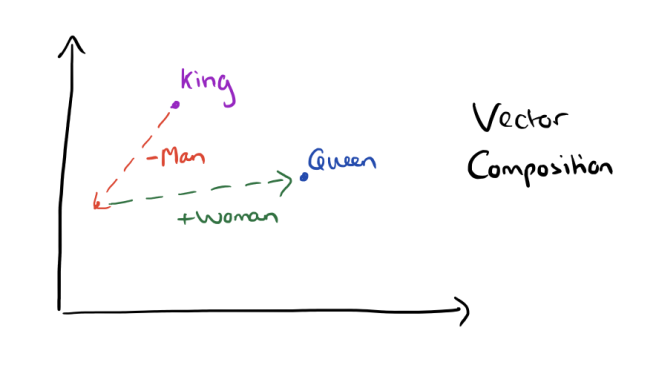
\includegraphics[height=5cm]{img/word2vec-king-queen-composition}
  \caption{Word2vec king queen composition}
\label{fig:word2vec_king_queen_composition}
\end{figure}

The most famous realization of these embeddings was introduced by the researchers of Google around Tomas Mikolov in their paper “Distributed Representations of Words and Phrases and their Compositionality“~\footcite{DBLP:journals/corr/MikolovSCCD13}. Hereafter, their proposed approach, Word2Vec, along with their used notation will briefly be presented, as its core ideas are found throughout other popular word embedding frameworks as well. \\
Given a sequence of training words $ w_1, w_2, \dots, w_T $, the objective (paragraph~\ref{par:cost_function}) is to minimize the average negative log likelihood
\begin{equation}
	\label{eqn:skip_gram_objective_function}
	J(\theta) = - \frac{1}{T} \sum_{t=1}^{T} \sum_{\substack{-m \leq j \leq m \\ j \neq 0}} \text{log} \ P(w_{t+j} | w_t; \theta)
\end{equation}
where $ m $ is the fixed window size containing the context words around the center word $ w_j $. Enlarging this window size results in more training examples and can lead to a higher accuracy, at the expense of training time. In order to compute the term $ P(w_{t+j} | w_t; \theta) $ a regular softmax function (ch 3.3.3 [HARDCODED, ref to softmax function]) can be applied
\begin{equation}
	\label{eqn:skip_gram_conditional_probability}
	P(o | c) = \frac{\text{exp} \ (u_{o}^{T} v_{c})}{\sum_{w \in V} \text{exp} \ (u_{w}^{T} v_c)}
\end{equation}
where we use two vectors per word $ w $: $ v_w $ when $ w $ is a center word and $ u_w $ when $ w $ is a context word. Optimizing the objective function results in high-quality distributed vector representations. It should be noted that for computational efficiency modified versions of these functions such as negative sampling or hierarchical softmax are used, as the presented ones do not scale well.

Even though word2vec embeddings are a powerful representation they do face certain limitations, which is why \textit{Stanford University}~\footnote{\url{https://www.stanford.edu}} took it upon itself to create an improved variant called GloVe~\footcite{pennington-etal-2014-glove}. While word2vec ignores that some context words appear more ofthen than others, GloVe stresses the importance of frequencies of co-occurrences and that these should not be “wasted“ as additional training examples. Therefore, GloVe builds word embeddings in a way that a combination of word vectors relates directly to the probability of these words' co-occurrence in the corpus. \\
Another alternative to word2vec is \textit{fasttext} by Facebook, which generates word vectors that generalize better, need less training data and can be trained “on more than one billion words in less than ten minutes using a standard multicore CPU, and classify half a million sentences among 312K classes in less than a minute“ according to the authors~\footcite{DBLP:journals/corr/JoulinGBM16}. FastText also takes word parts into account, i.e. FastText not only stays on a word level of depth but also goes into the character level.


\subsubsection{Foundations of language modeling}
\label{sub:foundations_of_language_modeling}

As the necessary preprocessing has been dealt with, we can now get to the actual task of language modeling, which is the task of predicting “what word comes next“. More formally, this means: Given a sequence of words $ x^{(1)}, x^{(2)}, \dots, x^{(t)} $, compute the probability of the next word $ x^{(t+1)} $:
\begin{equation}
    P(x^{(t+1)} | x^{(t)}, \dots, x^{(1)})
\end{equation}
where $ x^{(t+1)} $ can be any word in the vocabulary $ V = \{w_1, \dots, w_{|V|}\} $.  \\
Having a system that does so allows us to assign a probability to a text excerpt of length $ T $:
\begin{align}
    \begin{split}
    P(x^{(1)}, \dots, x^{(T)}) &= P(x^{(1)}) \times P(x^{(2)} | x^{(1)}) \times \cdots \times P(x^{(T)} | x^{(T-1)}, \dots, x^{(1)}) \\
    &= \prod_{t=1}^{T} P(x^{(t)} | x^{(t-1)}, \dots, x^{(1)})
    \end{split}
\end{align}
Developing and improving language models is a task central to language understanding by which we can measure how well machine learning systems actually comprehend natural language. This is demonstrated by the fact that “often (although not always), training better language models improves the underlying metrics of the downstream task (such as word error rate for speech recognition, or BLEU score for translation), which makes the task of training better LMs valuable by itself”~\footcite{DBLP:journals/corr/JozefowiczVSSW16}. \\
Since the first significant language model was proposed back in 1980~\footcite{880083}, language models and their architectures have gone through many changes. Especially the rise of deep learning and new network models such as recurrent neural networks (RNNs) or transformers have fueled language modeling research in the past few years.


\subsubsection{N-Gram models}
\label{sub:n_gram_models}

One solution in dealing with the problem of predicting a word after a sequence of $ (n - 1) $
words in the form of a Markov model, i.e. the probability of each event depends only on the state
attained through the previous event, is called an n-gram model. An “n-gram” hereby denotes a chunk 
of n consecutive words. The core idea is that the probability of a word $ w_i $ occurring in the 
$ i^{th} $ instance after a sequence of $ (i - 1) $ preceding words can be approximated by observing 
only the preceding context of $ (n - 1) $ words.

Following this insight we can compute the probability of all n-grams in a corpus of text by simply counting their occurrences.
Doing so allows us to calculate the conditional probabilities like so:
\begin{align}
    \begin{split}
        P(x^{(t+1)} | x^{(t)}, \dots, x^{(1)}) &= P(x^{(t+1)} | x^{(t)}, \dots, x^{(t - 2 + 2)}) \\ \\
        &= \frac{P(x^{(t+1)}, x^{(t)}, \dots, x^{(t - 2 + 2)})}{P(x^{(t)}, \dots, x^{(t - 2 + 2)})} \\ \\
        &\approx \frac{\text{count}(x^{(t+1)}, x^{(t)}, \dots, x^{(t - n + 2)})}{\text{count}(x^{(t)}, \dots, x^{(t - n + 2)})}
    \end{split}
\end{align}
N-gram models where $ n = 1 $, $ n = 2 $ and $ n = 3 $ are called unigram, bigram and trigram, respectively. The parameter $ n $ typically does not get bigger than $ 5 $. Having the conditional probabilites new text can be generated by conditioning on the provided input. After getting a probability distribution over the vocabulary a sampling strategy (ch. 3.3.3 [HARDCODED]) that returns a word has to be applied.

Even though n-gram models have been widely used especially due to their simplicity and scalability they do face certain limitations that have led to a decrease in their popularity. One problem that can occur is the one of unexpected n-grams: if the $ n $-gram encountered in the test setting did not appear in the corpus that the model was trained on, then the probability for the $ n^{th} $ word conditioned on the $ (n-1) $ words is $ 0 $. If an $ (n-1) $-gram is encountered in the test setting but not in the training data, then the model can not calculate the probability of any word that comes after. These two sparsity limitations can, however, partly be encountered by using smoothing and backoff techniques. The storage problem is evident, as increasing $ n $ or simply enlarging the training corpus increases the model size, which poses a significant problem for larger NLP applications. The implications of this restriction can be withdrawn from the following illustrative generated text snippet:

\begin{quote}
“today the price of gold per ton , while production of shoe lasts and shoe industry , the bank intervened just after it considered and rejected an imf demand to rebuild depleted european stocks , sept 30 end primary 76 cts a share”
\end{quote}

Because of the inability to expand the context window effectively, we remain tied to a LM that can generate grammatical but also incoherent model that can not relate predictions to history reaching further into the past. N-gram language models are still widely used in speech recognition due to their high efficiency in inference~\footcite{wang2019improving} but their limitations caused by poor generalization to unobserved n-grams and inability to capture long range dependencies led to the rise of neural language models.





\subsubsection{Neural language models}
\label{sub:neural_language_models}

\paragraph{Neural network}
This is some text.

\paragraph{Recurrent neural networks}
This is some text.

\paragraph{Convolutional neural networks}
This is some text.

\paragraph{Attention and transformers}
This is some text.

\subsubsection{Attention and transformers}
\label{sub:attention_and_transformers}

In their paper `Attention is all you need'~\footcite{DBLP:journals/corr/VaswaniSPUJGKP17} Google researchers around Ashish Vaswani introduced a new architecture reliant solely on attention mechanisms~\footcite{DBLP:journals/corr/LinFSYXZB17}, i.e. without any recurrence or convolution. Nonetheless, this `transformer' based architecture is superior in both quality and speed. Its structure allows for strong parallelization and thus requires significantly less time to train. Furthermore, transformers generalize well to other tasks, so that the same model can be utilized for multiple \gls{nlp} tasks. In this subsection, the main building blocks of the transformer architecture will be presented. As this architecture is fairly novel the amount of literature is very limited and the applied notation is heavily inspired by the original paper and by the blog post `Transformers from scratch'~\footnote{\url{http://www.peterbloem.nl/blog/transformers}}.

\paragraph{Self-attention}
Given are a sequence of input vectors $ \boldsymbol{x_1}, \boldsymbol{x_2}, \dots, \boldsymbol{x_t} $ and corresponding output vectors $ \boldsymbol{y_1}, \boldsymbol{y_2}, \dots, \boldsymbol{y_t} $, all of which have dimension $ k $. For the calculation of the output vector $ \boldsymbol{y_i} $, the self-attention mechanism takes a weighted average over all the input vectors
\begin{equation}
	\boldsymbol{y_i} = \sum_j w_{ij} \boldsymbol{x}_j
\end{equation}
where $ j $ indexes over the input sequence the sum of all weights is equal to $ 1 $. Unlike in other architectures, $ w_{ij} $ is not a parameter, but it is the result of a function over $ \boldsymbol{x_i}^T \boldsymbol{x_j} $. A simple form this function could take on would be that of the dot product:
\begin{equation}
	w'_{ij} = \boldsymbol{x}_i^T \boldsymbol{x}_j
\end{equation}
In order to get a value range of $ [0, 1] $ instead of $ (-\infty, +\infty) $ and a sum over all weights of 1, a softmax function is applied over the sequence of weights:
\begin{equation}
	w_{ij} = \frac{\text{exp} \ (w'_{ij})}{\sum_j \text{exp} \ (w'_{ij})}
\end{equation}

To give an intuition as to what is going on under the hood one might consider the input sentence ``she thinks about the exam''. After this sentence passes the typical embedding layer it turns into the vector sequence $ v_{\text{the}}, v_{\text{girl}}, v_{\text{thinks}}, v_{\text{about}}, v_{\text{the}}, v_{\text{exam}} $. Providing this vector sequence to an self-attention layer would result in an output sequence of vectors $ y_{\text{the}}, y_{\text{girl}}, y_{\text{thinks}}, y_{\text{about}}, y_{\text{the}}, y_{\text{exam}} $ where $ y_{\text{girl}} $ is a weighted sum over all the embedding vectominusculers in the first sequence, weighted by their normalized dot-product $ v_{\text{girl}} $. Now, as the definite article `the' is just used to introduce specific nouns, its presence will be probably of little relevance to the interpretation of other words in the sentence. Therefore, the embedding $ v_{\text{the}} $ will end up being a vector that has a minuscule or negative - in our case - dot product with other words. On the contrary the noun `girl' is important to determine the correct conjugation of the verb `thinks' - if the noun was `boys' instead the verb would have to be rewritten to `think'. This leads to the embeddings $ v_{\text{girl}} $ and $ v_{\text{thinks}} $ most likely having a large and positive dot product together. It is interesting to note at this point that self-attention regards the input as a \textit{set} instead of as a sequence, which means that the order of the words in the input sequence has no relevance; permuting the input sequence will generate the same $ y $-vectors. However, the order of the words is of course relevant to text processing tasks, which is why positional information of words will be integrated elsewhere. There are other components required for the complete transformer architecture, but self-attention is the only operation that transfers information between vectors. All other operations focus on solely processing one vector in the input sequence at a time.

For the sake of efficient computation and better data representation a few additional tweaks have to be implemented to get the final form of self-attention in a transformer. For starters, each input vector $ x_i $ is used thrice for self-attention: Once, to compare it to all other vectors to establish the weights for its own output $ y_i $. Then, to compare it to all other vectors in order to establish the weights for the output of each other vector $ y_j $ where $ j \neq i $. And one last time as part of the weighted sum to calculate each output vector once the weights have been established. Following the notation of the original paper these roles are called \textbf{query}, \textbf{key} and \textbf{value}. Unlike in the previous example where one vector played all three roles, in the real world three vectors are derived from one input $ x_i $:
\begin{equation}
	\boldsymbol{q}_i = \boldsymbol{W}_q \boldsymbol{x}_i \quad \boldsymbol{k}_i = \boldsymbol{W}_k \boldsymbol{x}_i \quad \boldsymbol{v}_i = \boldsymbol{W}_v \boldsymbol{x}_i
\end{equation}
where each weight matrix $ \boldsymbol{W} $ is of dimension $ k \times k $. The calculation of the final output vectors is done with
\begin{align}
	\begin{split}
		w'_{ij} = \boldsymbol{q}_i^T \boldsymbol{k}_j \\
		w_{ij} = \text{softmax} \ (w'_{ij}) \\
		\boldsymbol{y}_i = \sum_j w_{ij} \boldsymbol{v}_j.
	\end{split}
\end{align}
This separation grants the possibility to taylor the input vectors separately to these three roles. Besides that, the authors observed the problem of large dot products with an increasing dimension $ k $. To encounter this problem a scaling factor of $ \frac{1}{\sqrt{k}} $ was introduced into the calculation of the weights:
\begin{equation}
	w'_{ij} = \frac{\boldsymbol{q}_i^T \boldsymbol{k}_j}{\sqrt{k}}
\end{equation}
Lastly, the authors found it beneficial to use multiple attention layers side by side to ``attend to information from different representation subspaces at different positions''~\footcite[5]{DBLP:journals/corr/VaswaniSPUJGKP17}. This basically means that it is helpful to allow for a word to have different relations to different parts of the sentence. To account for this, several attention mechanisms (indexed by $ r $) called attention heads and with separate weight matrices $ \boldsymbol{W}_q^r, \boldsymbol{W}_k^r, \boldsymbol{W}_v^r $ are used.

\paragraph{Architecture}
\begin{figure}[h]
  	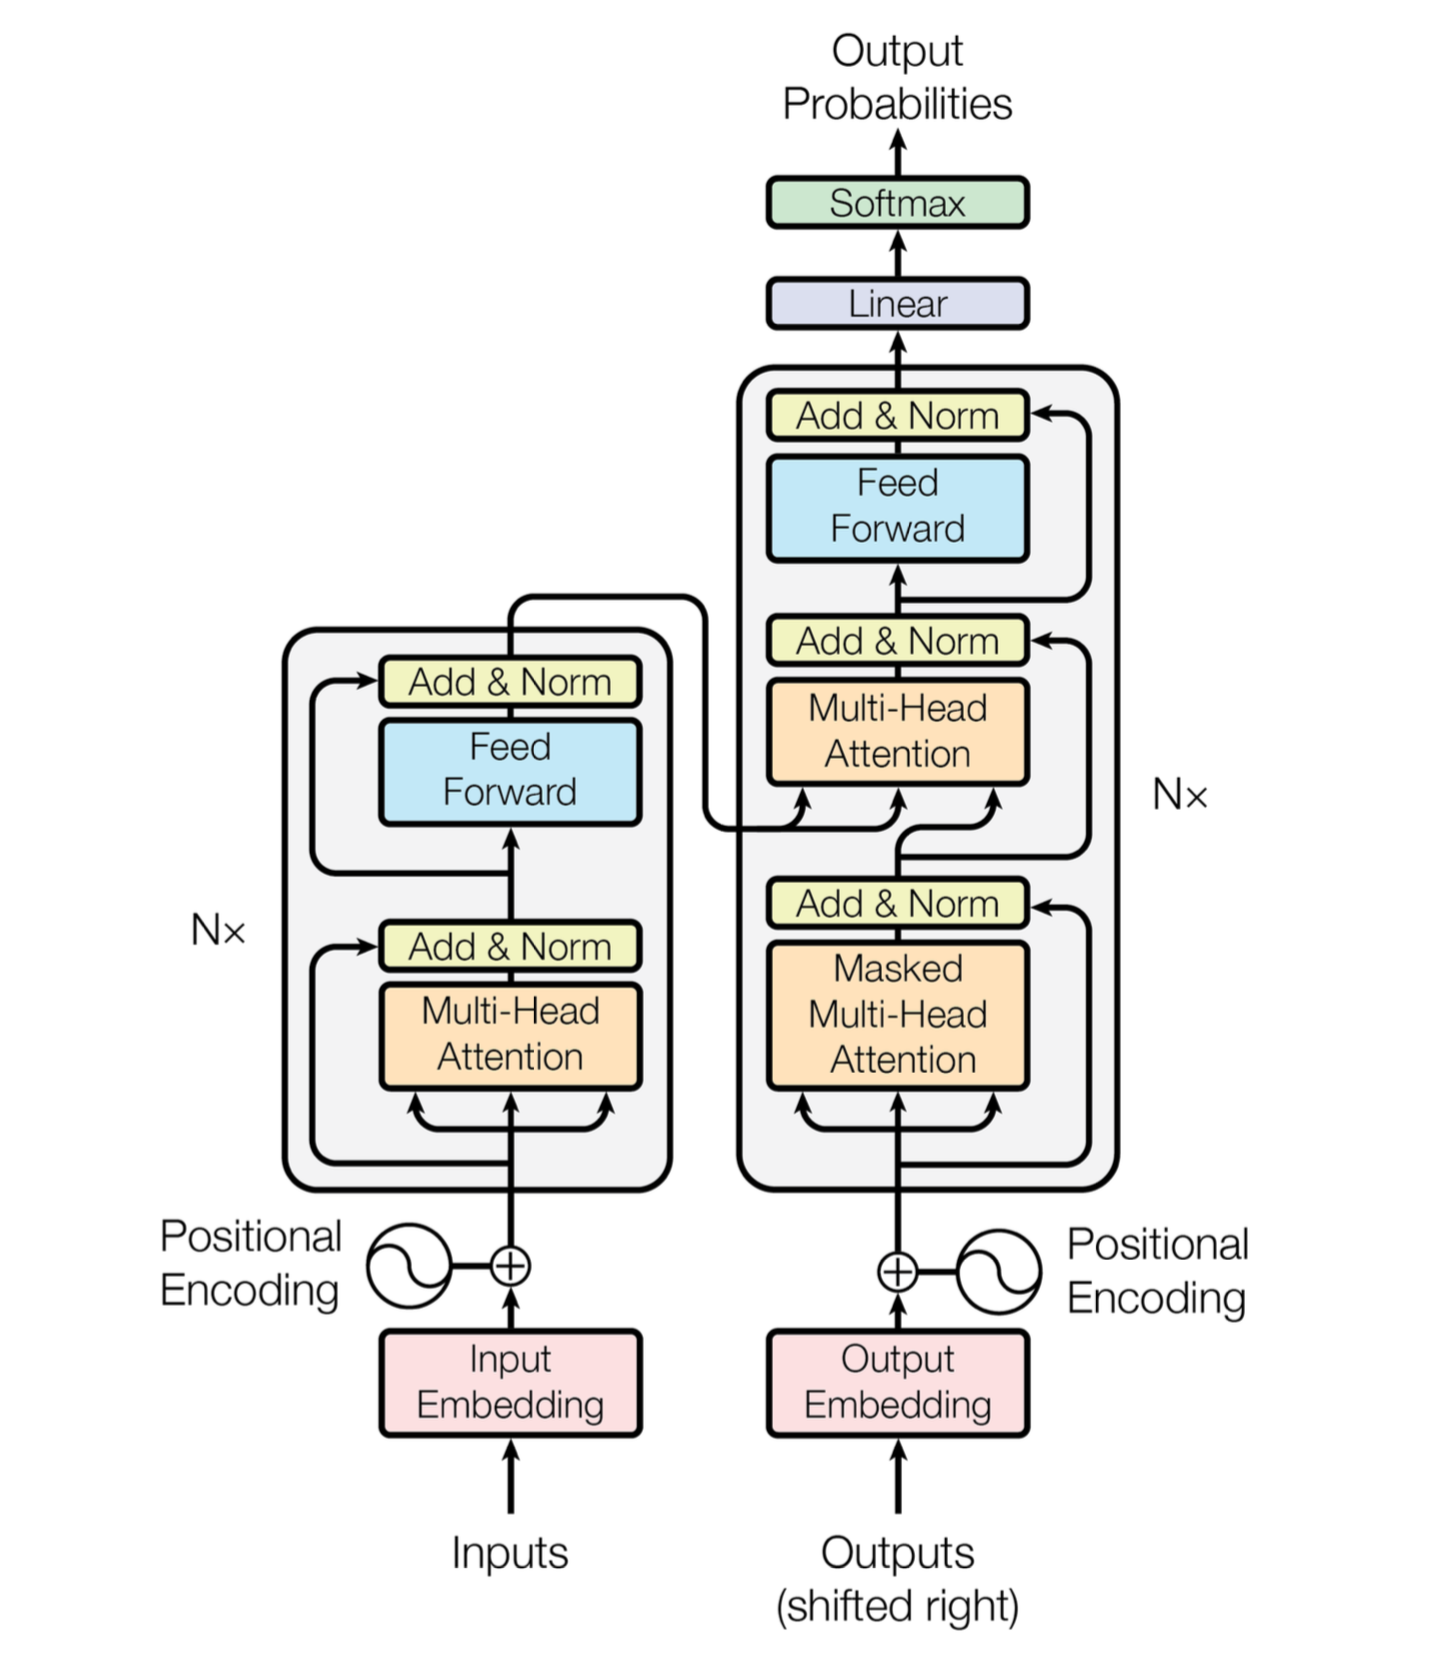
\includegraphics[height=12cm]{img/transformer}
  	\caption[Transformer model architecture]{Transformer model architecture~\footnote{\url{https://medium.com/inside-machine-learning/what-is-a-transformer-d07dd1fbec04}}}
	\label{fig:transformer}
\end{figure}
Figure~\ref{fig:transformer} shows the basic transformer architecture, which is fundamentally split up into the encoding stack on the left and the decoding stack on the right. A transformer block roughly consists of a self-attention (or multi-head-attention) layer, a layer normalization, a feedforward layer and finally another normalization layer. Residual connections are added before each normalization phase. Normalization and regularization techniques are commonly used to speed the training of deep models up and even improve their accuracy~\footcite{DBLP:journals/corr/abs-1903-00925}. After determining the input and output embeddings there is a preliminary step called \textbf{positional encoding}. As stated above, transformers do not contain recurrence or convolution. So, in order for the model to understand the ordering of the input sequence, information about either the relative or absolute position of the tokes in the sequence need to be injected. These positional encodings have the same dimension as the embeddings, so the two can be summed. The encodings are hereby not learned, but take on the form of some function $ f: \mathbb{N} \rightarrow \mathbb{R}^k $ to map the positions to real-valued vectors. For the original transformer, sine and cosine functions of different frequencies were utilized:
\begin{align}
	\begin{split}
		PE_{pos, 2i} = \text{sin} \ \left( \text{pos} \ / 10000^{2i / k} \right) \\
		PE_{pos, 2i + 1} = \text{cos} \ \left( \text{pos} \ / 10000^{2i / k} \right)
	\end{split}
\end{align}
These functions were chosen, as the researches hypothesized that they would allow the model to easily learn to attend by relative positions, since for any fixed offset $ o $, $ PE_{pos + k} $ can be represented as a linear function of $ PE_{pos} $. Another advantage of choosing functions rather than learning positional embeddings stems from the fact that the model can learn to extrapolate to sequence lengths longer than the  ones encountered during training. After calculating the embeddings, adding the positional encodings and passing the encoder and decoder stacks, a learned linear transformation is used and afterwards a softmax function applied to convert the decoder output to predicted next-token probabilites. In order to actually predict the next word, a sampling strategy needs to elect one from the final probability distribution.



\subsubsection{Autoencoders and autoregressors}
\label{sub:autoencoders_and_autoregressors}

While most current \gls{lm}s are based on the transformer architecture they differ in their approach of predicting new tokens for the task of language modeling. Models like \gls{gpt2} make use of \textbf{\gls{ar}} language modeling while others employ \textbf{\gls{ae}} for language modeling.

\begin{align}
	\label{eq:bayes_theorem}
	\mathbin{\textcolor{red}{p(\Theta|D)}} = \frac{\mathbin{\textcolor{blue}{P(D|\Theta)}} \ \mathbin{\textcolor{orange}{P(\Theta)}} }{P(D)} \quad \rightarrow \quad
	\textcolor{red}{\text{posterior}} \propto \textcolor{blue}{\text{likelihood}} \times \textcolor{orange}{\text{prior}}
\end{align}

To understand these two concepts of prediction, one first needs to distinguish between generative and discriminative predictor models. While the complicated background to these approaches divides the research community (\textit{``Bayesian vs. Frequentist inference''}), one must hereof only understand that both have the same goal of predicting the class posterior probability of their input (equation~\ref{eq:bayes_theorem}). The actual calculation, however, is performed in two distinct ways. Generative predictor models try to understand the distribution of the underlying distribution of the data. Herefore, they estimate the likelihood $ P(D|\Theta) $ as well as the prior $ P(\Theta) $ and together with the evidence $ P(D) $ compute the class posterior probabilities. Discriminative predictor models learn their decision boundaries by directly computing the posterior from the training data and thus do not try to understand the underlying distribution. Discriminative models are easier to learn in general because they do not need to learn the actual distribution of each class. Instead, they focus only on finding their differences. They are computationally less complex and therefore model fewer probabilities than generative ones.

Generative models currently form the basis of natural language understanding and are responsible for recent research breakthroughs. Unsupervised representational learning methods, when pretrained with unlabeled corpora and then fine-tuned for downstream tasks, can be either implemented as \gls{ar} or \gls{ae} language modeling. To highlight the difference between these two, one can take a look at their way of predicting an unknown token in a sequence of text:
\begin{equation}
	\dots, x_{t-2}, x_{t-1}, x_{t, \text{prediction}}, x_{t+1}, x_{t+2}, \dots
\end{equation}
\gls{ar} language modeling (e.g. in \gls{gpt2}) can only predict new tokens in one direction. For the given token sequence of length $ T $ it computes the text probability as either a \textit{forward} $ p(x) = \prod_{t=1}^{T} p(x_t | x_{<t}) $ or \textit{backward} $ p(x) = \prod_{t=T}^{1} p(x_t | x_{>t}) $ product. This means that the foremost (or last) token is computed sequentially, taking the previously calculated tokens into account for the predicition at each step. In comparison, \gls{ae} based pretraining does not perform a density estimation, but instead aims to reconstruct the original data from \textit{masked} (hidden) inputs. Usually, some form of noise is inserted into the sequence and the model is trained to reconstruct the original sequence from the corrupted version. Since density estimation is not part of the goal, the \gls{ae} model may use the context to both sides (in the above sequence: $ \dots, x_{t-2}, x_{t-1} $ \textit{and} $ x_{t+1}, x_{t+2}, \dots $) for reconstruction. Nonetheless, the artificial noise inserted during the \gls{ae} pretraining usually is missing in the real data during the fine-tuning process. This commonly leads to a discrepancy between pretraining and fine-tuning. Unlike \gls{ar} models, \gls{ae} models cannot model the probability using the product rule.


\subsubsection{Current language models}
\label{sub:current_language models}

OpenAI made headlines when it first announced the creation of a language model so powerful that it led them to not release it due to ``concerns about malicious applications of the technology''~\footnote{\url{https://openai.com/blog/better-language-models/}}. \gls{gpt2} is a large transformer-based language model with about 1.5 billion parameters, trained on a dataset of 8 million web pages, or 40GB of raw text data~\footcite{radford2019language}. Creators of the \gls{gpt2} model intentionally trained their model on a diverse basis of text in order to produce a \gls{lm} that could generalize well to many different tasks (``zero-shot'' setting) across diverse domains (table~\ref{tab:gpt2_benchmark_scores}) - even outperforming \gls{lm}s trained on specific domains like news or books without needing to use those domain-specific training datasets. What mainly caused the enthusiasm for this model was the fact that it could generate text samples of high, human-like quality and at the same time maintain coherence across long passages of text. After some time passed, OpenAI decided to publish their code, the weights and the training dataset in the form of a staged release. On November 2019, OpenAI released the largest form of their model, also called `GPT-2-XL', consisting of 1.5 billion weights following their releases of the 117M, 345M and 762M parameter-sized models, making it publicly accessible and usable by everyone~\footnote{\url{https://github.com/openai/gpt-2-output-dataset}}.

\begin{table}
	\centering
	\caption{Excerpt of the GPT-2 zero-shot results on different datasets and with different model sizes}
	\begin{tabular}{ cccccccccc }
		\hline
		& LAMBSDA & CBT-CN & WikiText2 & PTB & enwik8 & text8 & WikiText103 & 1BW \\
		& (PPL) & (ACC) & (PPL) & (PPL) & (BPB) & (BPC) & (PPL) & (PPL) \\ \hline
		SOTA & 99.8 & 85.7 & 39.14 & 46.54 & 0.99 & 1.08 & 18.3 & 21.8 \\ \hline
		117M & 35.13 & 87.65 & 29.41 & 65.85 & 1.16 & 1.17 & 37.50 & 75.20 \\
		345M & 15.60 & 92.35 & 22.76 & 47.33 & 1.01 & 1.06 & 26.37 & 55.72 \\
		762M & 10.87 & 93.45 & 19.93 & 40.31 & 0.97 & 1.02 & 22.05 & 44.575 \\
		1542M & 8.63 & 93.30 & 18.34 & 35.76 & 0.93 & 0.98 & 17.48 & 42.16 \\ \hline
	\end{tabular}
	\label{tab:gpt2_benchmark_scores}
\end{table}

Currently there are several language models that are actively being worked on and at the disposal of researchers and interested parties. Especially pretrained models such as \gls{bert}, \gls{gpt2} and XLNet have been known to perform particularly well across common \gls{nlp} tasks. \gls{bert} for instance achieved SotA-scores for Question Answering (SQuAD v1.1), Natural Language Inference (MNLI), and other tasks~\footcite{DBLP:journals/corr/abs-1810-04805}. It is worth noting that both \gls{gpt}-2 as well as \gls{bert} are built on top of the aforementioned transformer architecture proposed by Vaswani and colleagues (subsection~\ref{sub:attention_and_transformers}). \gls{bert} hereby uses the transformer-encoder stack and \gls{gpt2} uses the transformer-decoder stack. The XLNet model presented in mid-2019~\footcite{DBLP:journals/corr/abs-1906-08237} is based on the decoder blocks of a further development of the transformer: Transformer-XL, which extends the transformer architecture by a recurrent connection and a different positional coding~\footcite{DBLP:journals/corr/abs-1901-02860}. \gls{bert} can learn bidirectionally, \gls{gpt}-2 and XLNet unidirectionally using the autoregressive approach. XLNet additionally uses permutation to obtain n representations of the sequence. This allows the model to combine the advantages of autoregression and autoencoding.

Wang and Cho conducted a scientific comparison between the LM performance of the predecessor of \gls{gpt}-2 and \gls{bert}~\footcite{wang2019bert}. The work empirically proves a better quality of \gls{gpt} generation. In contrast, XLNet has recently shown SotA results for problems outside the standard LM task. A scientific comparison of \gls{gpt}-2 and XLNet regarding the classical text generation capability has not yet been made. When comparing the AI community and juxtaposing them in the context of this thesis, the text generation of XLNet seems to be somewhat more coherent, but more often shows grammar errors. Overall, the output of \gls{gpt}-2 slightly exceeds that of XLNet. However, empirical comparisons are necessary to confirm this hypothesis. Another transformer model was recently posted on the GoogleAI blog~\footnote{\url{https://ai.googleblog.com/2020/01/reformer-efficient-transformer.html}}. This transformer is said to have a context window that extends to thousands of words and can thus be used to generate entire Wikipedia articles through multi-document summarization. Google AI researchers believe that the Reformer gives ``the basis for future use of Transformer models, both for long text and applications outside of natural language processing''~\footcite{kitaev2020reformer}. However, as this model was published at the time of an advanced stage of this thesis and as there was no PyTorch implementation of the pretrained model at the time in question, it was not further considered for this thesis. Consequently, the \gls{gpt2} model will be used to generate the text snippets necessary for the later proposed dataset. It is worth mentioning that these \gls{lm}s are freely available to the public. More powerful models created by big tech companies such as the Nvidia \textit{Megatron} with 8.3 billion or the Microsoft \textit{NLG-Turing} with 17 billion parameters do exist (figure~\ref{fig:lm_model_comparison}) but as they are disclosed to the public, no statements can be made about their performance and suitability for this work.
\begin{figure}[h]
  	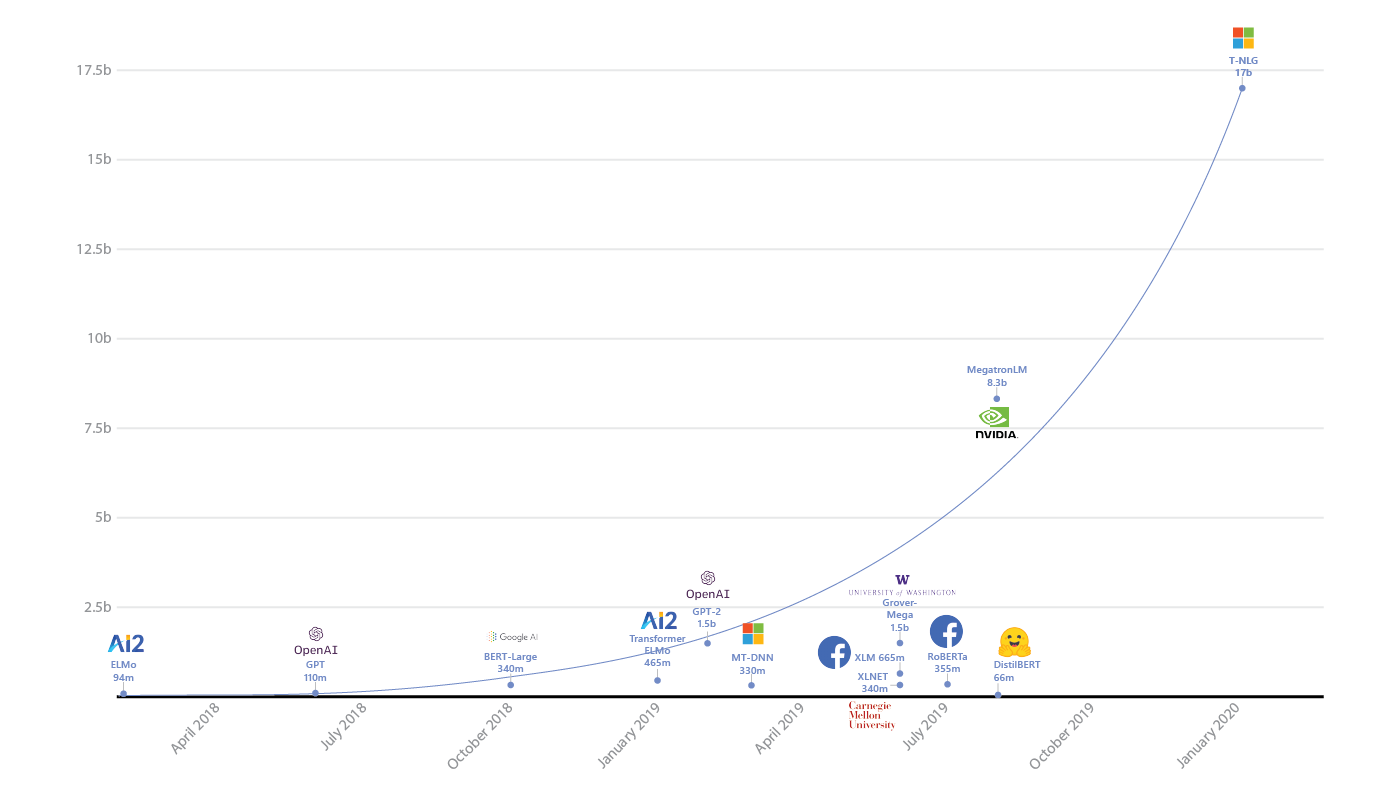
\includegraphics[height=8cm]{img/lm_model_comparison}
  	\caption{Comparison of language model sizes}
	\label{fig:lm_model_comparison}
\end{figure}


\subsection{Related Work}
\label{sec:related_work}

After having established necessary background knowledge and before heading into the methodolgy (ch.~\ref{ch:methodology}), this section examines related work to the detection of synthetically generated text. Because of the novelty of the problem the existing approaches are not only rare, but also vary significantly in their approaches to solve the problem as well as in their extensiveness - some are frameworks that merely formulate the detection of a language model output as a hypothesis testing problem while others provide out-of-the-box tools to be instantly used over text. The one thing that current research does have in common, is the pure focus on the text content to discriminate between genuine and generated text. Approaches that narrow down a domain and benchmark classification methods with the addition of domain-specific information (metadata) have not been published yet.

\subsubsection{Giant Language model Test Room}
\label{sub:gltr}

\gls{gltr}~\footcite{DBLP:journals/corr/abs-1906-04043} is the result of a collaboration of \textit{MIT-IBM Watson AI lab}~\footnote{\url{https://mitibmwatsonailab.mit.edu/}} and \textit{HarvardNLP}~\footnote{\url{http://nlp.seas.harvard.edu/}} with the goal of providing a tool to support non-expert humans in detecting whether a text was generated by a model or not. The authors see many paths for malicious actors to abuse current \gls{lm}s for the purpose of generating fake reviews, comments or news articles and thereby influencing the public opinion. In their work, the authors argue that the \gls{lm}s' ways of working are prone to be detected by simple statistical methods when used as a visual assisstance tool. The core assumption is that systems over generate from a restricted subset of the true distribution of natural language, for which they have high confidence. While one might argue that this approach will only be successful if access to the system distribution is provided, Gehrmann and Strobelt hypothesize that these methods generalize well to black-box scenarios, as long as the synthetic text follows a similar sampling strategy than that of a large language model. GLTR assists its users by highlighting sequences that are very probable and unsurprising with green and yellow colors and sequences that are rather unlikely and uncommon with purple and red colors (figure~\ref{fig:gltr}).

\begin{figure}[h]
  	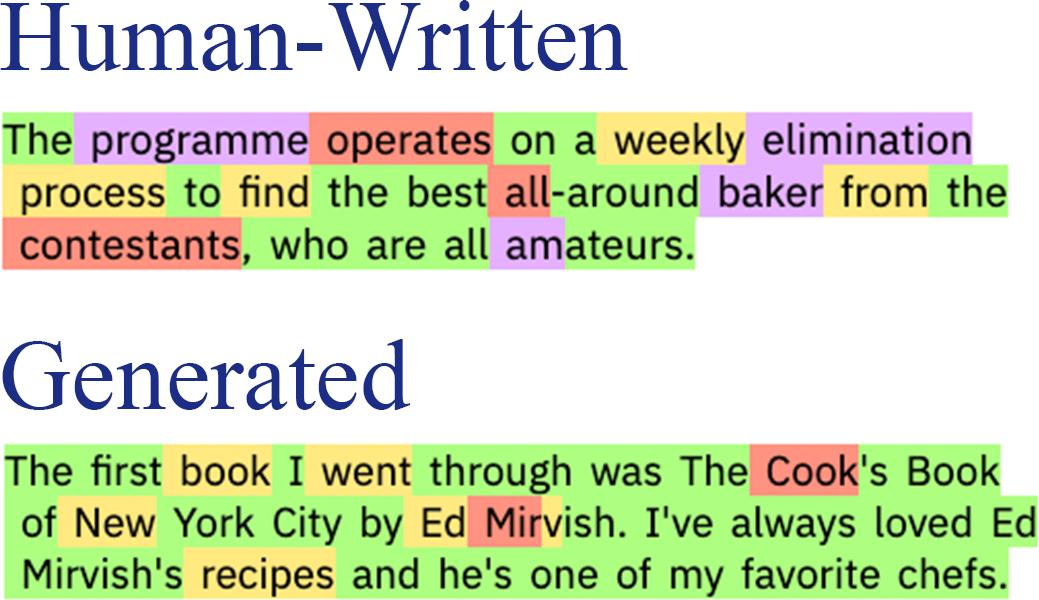
\includegraphics[height=5cm]{img/gltr}
  	\caption{GLTR visualization}
	\label{fig:gltr}
\end{figure}

In order to calculate the likelihood of text, \gls{gltr} applies three different tests: \textbf{Test 1} computes the probability of the word $ p_{\text{det}}(X_i = \hat{X}_i | X_{1:i-1}) $. \textbf{Test 2} computes the absolute rank of a word, e.g. rank in $ p_{det}(X_i | X_{1:i-1}) $ and \textbf{test 3} computes the entropy of the predicted distribution, e.g. $ - \sum_w p_{\text{det}}(X_i = w | X_{1:i-1}) \ \text{log} \ p_{\text{det}}(X_i = w | X_{1:i-1}) $. The first two tests check whether a generated word is sampled from the top of the distribution and the third test checks if the preceding context is well-known to the detection system such that it is sure of its next prediction. By default, a word that ranks within the top 10 is highlighted in green, top 100 in yellow, top 1,000 in red, and the rest in purple. The results of a conducted human-subjects study showed that \gls{gltr} improved the human detection-rate of fake text from 54\% to 72\% without any prior training. While an adversarial schme might try to fool \gls{gltr}, it would be forced to sample from the tail of the distribution and thus risk decreasing coherence of a text which makes it in turn easier for a human to identify the synthetic text. A significant limitation, however, results from the fact that a hidden seed text might be utilized to condition the sample distributions. Then, a conditional distribution will be different, even if \gls{gltr} has access to the model. While \gls{gltr} has this shortcoming, the authors are confident that their tool might be used to e.g. assist moderators on social media or review platforms.


\subsubsection{Grover}
\label{sub:grover}

In their paper~\footcite{zellers2019neuralfakenews} the authors present a model for controllable text generation called \textbf{Grover}. This model can generate article-like texts when prompted with a headline like `Why Bitcoin is a great investment' (figure~\ref{fig:grover}).

\begin{figure}[h]
  	
\includegraphics[height=7cm]{img/grover_fake_article}
  	\caption{Fake article excerpt, written by Grover}
	\label{fig:grover}
\end{figure}

This means, Grover was specifically designed to articles - these have a necessary structure beyond the pure text, or the body field. Other fields include the domain of the article and relating thereto the style of the artcile, the date of the publication, the names of the authors and the headline. In this sense, an article can be modeled by the joint distribution
\begin{equation}
	p(\text{domain}, \text{date}, \text{authors}, \text{headline}, \text{body}).
\end{equation}
As for the architecture, Grover uses the same one as \gls{gpt2} and comes in three different versions: Grover-Base with 124 million parameters, Grover-Large with 355 million parameters and Grover-Mega with 1.5 billion parameters. Grover was trained on the dataset `RealNews' which was presented by the authors and which consists of a large corpus of news articles from Common Crawl - being 120GB of size after deduplication. With the use of 256 TPU v3 cores, training time was two weeks. \\
Because most human-written articles found online are from the distant past, articles to be detected will likely be set in the present, which is why the authors frame neural fake news detection as a semi-supervised problem. To test the quality of generated articles news articles where split into four different categories: human-written articles from reputable news websites (short: `\textit{Human News}'), Grover-written articles conditioned on the same metadata (short: `\textit{Machine News}'), human-written articles from known propaganda websites (short: `\textit{Human Propaganda}') and lastly Grover-written articles conditioned on the propaganda metadata (short: `\textit{Machine Propaganda}'). When asking a pool of qualified workers on \gls{mturk} to distinguish between machine and human written text, results show that while the quality of Grover-written news is not as high as human-written news, Grovers is adept at rewriting propaganda: The workers on \gls{mturk} rated the trustworthiness scores of Grover propaganda higher than that of human propaganda. Talking about the future progress in discrimination, the authors say that their discriminators are effective, but they have the limitation that they rely primarily on distributional features of the content rathen than evidence. They argue that in contrast, humans assess whether an article is truthful by relying on a model of the world, revising whether the evidence in the article matches that model. That is why future work should investigate integrating knowledge into the discriminator.


\subsubsection{Other work}
\label{sub:other_work}

After releasing their own 1.63 billion-paramter \gls{lm} \gls{ctrl} which provides users with a fine-grained control over text generation~\footcite{keskar2019ctrl}, the Salesforce Research team also decided to tackle the tasks of classifying text as `genuine' or `generated'. In their paper ``Limits of Detecting Text Generated by Large-Scale Language Models''~\footcite{varshney2020limits} they present their framework [DETAILS ABOUT FRAMEWORK MISSING]. Besides that, several other studies have used supervised learning to develop classifiers for this task.
Solaiman et al.~\footcite{solaiman2019release}, the publishers of \gls{gpt2} as well as different members of the \gls{ctec} and others released a `manifest' in which they discuss the benefits of a staged release and propose guidelines to enhance coordination and responsibility in \gls{ai}. According to this work, there should be enough time in between model releases in order to be able to conduct risk and benefit analyses. Furthermore, the authors found out that the detection accuracy of current \gls{lm}s can be very sensitive to the sampling method of the test examples, depending on which sampling method the training examples used.
Another paper~\footcite{DBLP:journals/corr/abs-1906-03351} proposes the use of an \gls{ebm} framework (i.e. based on generative models). Its authors argue that because \gls{ebm}s are not limited to scoring a single word at a time these models might prove to be better detectors of generated text than auto-regressive models. In addition to that, \gls{ebm}s achieve good generalization when trained on large datasets.
Researchers at the \gls{mit} acknowledge recent studies on automatic fake news detection that either base their detection on the provenance of the article or that analyze the content and verify it against reliable sources, but they find that these approaches do not take account for the scenario where generators are also used for producing legitimate text, nor for more sophisticated attackers that use a generator to create malicious content while at the same time keeping minimal distributional differences from a legitimate source. To highlight this fact, Schuster et. al demonstrated the ineptitude of current detectors by considering auto-completion of news articles with correct information and also by considering an attacker that uses probabilites assigned by a language model to guide minimal edits that modify the correctness of an article's statements. Hereby, defenses that perform detection of auto-generated extremely well can be deceived by generator-based attackers. The authors therefore conclude that it is of utmost importance to develop better detectors against \textbf{all} types of fake news by e.g. building up diverse and challenging datasets. They also recommend the creation of a benchmark that represents content's veracity in a wide range of human-machine collaboration applications - taking not only whole article generation into consideration, but also hybrid writing and editing. According to them, it is more important to inspect potential fake news for veracity rather than provenance.
The paper ``Human and Automatic Detection of Generated Text''~\footcite{ippolito2019human} thoroughly investigates which choices such as sampling strategy and text excerpt length can impact the performance of not only automatic detection methods, but also human raters. Their findings suggest that there is a trade-off between automatic discriminator detection rate and human detection rate. For the automatic discriminator detection they first employed simple discriminators, such as bag-of-words or token likelihood bucketing which performed significantly worse than the use of a fine-tuned deep classifier such as \gls{bert}. After comparing the results of their fine-tuned classifier with the results annoted by humans the researchers conclude that current \gls{lm}s are able to generate text that is difficult for humans to detect, or difficult for discriminator to detect, but not necessarily both. They especially see a limitation in the fact that it is difficult for \gls{lm}s to generate text that is both exciting (i.e. unlikely) and semantically sound at the same time.



\section{Methodology}
\label{ch:methodology}

Having established the necessary background knowledge in the previous chapter, experiments undertaken in this thesis can  now be introduced. Section~\ref{sec:dataset} will introduce the dataset and its building process. Then, section~\ref{sec:approach} will describe the applied discriminator models.

\subsection{Dataset}
\label{sec:dataset}

In order to create a dataset suited for the classification task a few aspects had to be considered. \\
As deep learning methods with many parameters were going to be used for the classification task, many labeled training samples were needed. The dataset should ideally be comprised of equal amounts of synthetically and human-generated texts in order to not be biased towards a certain class and thus improve the accuracy of training. The first idea was to look for already built datasets that are freely available as these would not only reduce the time and amount of work needed for the creation of the dataset but also provide a benchmark against other models used on them. Because the examined classification task is fairly novel and powerful language models have just started to emerge in recent years, there is a lack of standardized data sets - prior research often focused on the detection of artificially generated academic papers instead of short texts~\footcite{lavoie2010algorithmic}. Furthermore, the incentive of using metadata related to text snippets and inspecting the changes in detection accuracy through it led to the motivation of building a new dataset. For this purpose, the following sources of human-created text were inspected - taking different aspects like data availability, extensibility by metadata, the potential for use of text generation and minimal overlap with the pretrained GPT2 Model into account: Wikipedia, Twitter, reviews (e.g. Amazon, IMDb), Reddit comments and news from the Reuters corpus.

With everything taken into consideration, Wikipedia articles were chosen as the best fit for this work. Reasons for this choice were the ease of access, the vast amount of data entries (currently there are more than 6 million articles in the English Wikipedia\footnote{\url{https://en.wikipedia.org/wiki/Wikipedia:Size_comparisons\#Wikipedia}}), the extensibility by metadata such as pageviews or categories and most importantly the fact that the ready-to-use GPT-2 model was explicitly not trained on any Wikipedia article since "it is a common data source for other datasets and could complicate analysis due to overlapping training data with test evaluation tasks."~\footcite[3]{radford2019language}. The reviews and Reddit comments datasets were not chosen because the metadata was not seen as decisive in improving detection quality. The disadvantage of the Reuters Corpus was that the training dataset used for the ready-to-use GPT2 model is comprised of many newspaper sources and thus is more likely to generate results that are rather similar to their human written counterparts. Twitter was seen as a promising data source, but the access to its public API was ended which is why it could not be further considered.

\subsubsection{Extraction Process}
\label{sub:extraction_process}

The two usual ways of scraping Wikipedia articles and other data like article metadata or media files from the Wikimedia Foundation\footnote{\url{https://wikimediafoundation.org/}} are through the APIs or the database dumps provided by the MediaWiki platform\footnote{\url{https://www.mediawiki.org/wiki/MediaWiki}}.
Both of these channels were used for different purposes:
The \textbf{database dumps} in the form of 17GB of compressed XML files were firstly downloaded and then titles, clear text and article ids were extracted using a python library called WikiExtractor\footnote{\url{https://github.com/attardi/wikiextractor}}. The output was stored in “.jsonl” (JSON lines) files, where each line denotes a complete JSON object. As the total size of the required metadata is a lot smaller, the \textbf{MediaWiki API} was used to retrieve information such as page views, the latest edit timestamp and categories linked to each article via the extracted article ids. Furthermore the API was used to access the latest news listed in WikiNews to generate exemplary news messages.

The extension of text samples by metadata was done for the purpose of examining three different hypotheses. \textbf{Firstly}, the assumption is being made that the detection rate varies (significantly) across different categories. \textbf{Secondly}, it is expected that the higher the edits and/or views on a page are, the lower the detection rate will be as the human text will be more sophisticated and better worded. \textbf{Thirdly}, the more recent the last edit timestamp of an article is, the lower the detection rate will be as newer information will be less likely to be present in the training data used for \gls{gpt2}. Furthermore, only articles with a minimum length of 1000 characters were taken into consideration as a measure to prevent a decrease in dataset quality (e.g. to filter out entries that only have a redirect notice to another article). For each article entry the last edit timestamp, the aggregated amount of page views over the last 60 days and the namespace was retrieved.

% \begin{itemize}
%     \item{\textbf{Database Dumps:}} Titles, clear text and article ids were extracted using a python library called WikiExtractor\footnote{\url{https://github.com/attardi/wikiextractor}}. MediaWiki provides Wikipedia database dumps in form of compressed XML files can be downloaded and then parsed by WikiExtractor. The output is stored in “.jsonl” (JSON lines) files, where each line denotes a complete JSON object.
%     \item{\textbf{Api:}} The MediaWiki API was used to retrieve metadata such as page views, the latest edit timestamp and categories linked to each article via the extracted page ids, but also to access the latest news listed in WikiNews to generate exemplary news messages.
% \end{itemize}

\subsubsection{Generation Parameter Combination}
\label{sub:generation_parameter_combination}

The output style of GPT2 differs depending on the chosen parameter combination. The parameters that influence the produced output the most are:
\begin{itemize}
    \item Input length
    \item Maximum output length
    \item Temperature - a higher value produces a softer probability distribution over classes which leads to “crazier” or more unlikely text, 
    whereas a lower value does the opposite [cite Hinton Paper no. 23]
    \item Repetition Penalty
\end{itemize}

In order to determine a parameter combination that generates convincing text all possible permutations between the parameters given the values 
listed in [ref table] were used to generate samples for 50 articles. As a metric for evaluation a fine-tuned large (1.5GB weights size as a .pt file) 
RoBERTa-based model with a mixture of temperature 1 and nucleus sampling outputs was chosen. This configuration was elected as it generalizes well 
to outputs generated using different sampling methods [citation gpt2 paper]. On top of that, human evaluation was performed while reading through 
samples created by the best performing parameter combinations according to the RoBERTa evaluation. \\
The main findings were that a higher repetition penalty as well as shorter output length were key factors for better text generation. In 
addition to that, choosing a lower temperature such as [cite Harvard paper] and feeding the LM word split input sentences as opposed to 
character split input sequences (“tennis is a sport” instead of “tennis is a spo”) also improved quality.

[show examples]

The finally selected parameter values were:

\paragraph*{Maximum Input Length - 60 characters}
The input that was fed into GPT-2 XL was the first sequence of plain text in a Wikipedia article, i.e. no infobox or content table text was 
considered. Additionally, before feeding the 60 character String into the LM it was split at the last word. This was done because the quality 
of the generated output tended to increase when input was given in full words rather than in characters and thus having many times split words.

\paragraph*{Maximum Output Length - 50 Tokens}
This corresponds to an average of about 240 - 260 characters per text (in comparison: the max tweet length is 280 characters). As this is a 
size that occurs a lot especially in social media or breaking news headlines (with the subtitle), the focus was placed on shorter text 
snippets [cite techcrunch and socialreport]. 
[insert figure that shows average character length per platform that achieves the best ‘virality’]

\paragraph*{Temperature - 1.0}
Both lowering and increasing (to 0.7 and 1.3) the temperature led to an increased detection of synthetically generated text, which is why 
the temperature was left at its original value.

\paragraph*{Repetition Penalty - 1.3}
As repetitions were not desired in the generated output the repetition penalty was increased from its default value of 1.0 to 1.3. Under the 
assumption that most Wikipedia articles do not contain repetitions (especially in their abstracts) unlike for instance dramatic text, where text 
repetition can be used as a stylistic device.

\paragraph*{Number of beams - 5}
Initially thought of as a parameter that would have a big impact on the quality of the generated text, it was found out that altering the number 
of beams used in the beam sampling strategy when predicting the next most probable tokens was had only little impact on the LM text generation. 
The values chosen ranged between 5 and 10 as this is currently the de facto standard [cite Stanford lectures] in research.


\subsection{Approach}
\label{sec:approach}

After setting up the dataset, the task of detecting synthetic text remains. Hereby, this thesis puts a particular emphasis on comparing the performance of classification methods throughout all complexity levels. To achieve this, available models were split into three different categories: In \textbf{category 1}, a first baseline using more elemental statistical models such as a \textit{logistic regression} or a \textit{\gls{svm}}. Here, the discriminator methods were we based upon features grounded in practice, that have been used in research throughout many years, such as \textit{TF-IDF} scores. The ideas for the use of these features and for the model architectures were taken from previous papers that dealt with this subject~\footcite{lavergne2008detecting,beresneva2016computer}. Having set up this baseline, \textbf{category 2} includes neural architectures that are specifically designed to process sequence input data. These models (\gls{rnn}, \gls{lstm}, \gls{cnn}, Transformer) employ complex neural layers which should result in the possibility to build more complex input representations and therefore also achieve a higher detection rate. Including the whole text as an input feature requires some preprocessing steps detailed in subsection~\ref{sub:word_representation}, mainly the tokenization of words and then the transformation into word embeddings. \textbf{Category 3} consists of the most complex detectors of currently available \gls{lm}s which were fine-tuned for the detection for the detection of the generated content. Firstly, by only providing text and later on by also providing the additional metadata. Because of their specialization, it is expected that these fine-tuned \gls{lm}s will perform best.

Like with the dataset creation process, most of the `explorative programming' was done in either local jupyter notebooks or Google Colaboratory. Especially the descriptive analysis process which requires no GPU-intensive tasks was done locally. The linear models and the deep feedforward networks were mainly trained on Google Colaboratory and the sophisticated ~\gls{lm}s were fine-tuned using the existing Google Cloud infrastructure mentioned above.

\subsection{Infrastructure}
\label{sec:infrastructure}

The dataset creation and the experiments were conducted using infrastructure suitable to handle complex computations and large datasets. The text generation process of \gls{lm}s as well as the training of deep neural networks typically requires the parallelizable computing power of graphics processors. In addition, large data files need to be stored and processed. To create the dataset given the aforementioned parameter configurations (subsection~\ref{sub:generation_parameter_combination}), the first pipeline runs took place in Google Colaboratory\footnote{\url{https://colab.research.google.com/notebooks/intro.ipynb}}, a free jupyter notebook cloud hosting platform which provides users with a GPU, in this case, an Nvidia Tesla K80\footnote{\url{https://www.nvidia.com/en-gb/data-center/tesla-k80/}}. For the generation of synthetic text, the large GPT-2 model (774M parameters) was used. The generation of each text snippet took about 11 seconds. As soon as the pipeline was fully functioning the jupyter notebooks were converted into python modules and the code was transferred to a Google Cloud\footnote{\url{https://cloud.google.com/}} deep learning virtual machine\footnote{\url{https://console.cloud.google.com/marketplace/details/click-to-deploy-images/deeplearning?_ga=2.99839453.-2121832178.1549923708}} (VM) with 13GB of memory, a 100GB standard persistent disk, and 2 Nvidia K80 GPUs. Google Cloud was elected for the reason of providing users with a free credit of 300\$, while other cloud computing providers such as AWS\footnote{\url{https://aws.amazon.com/}} or Azure\footnote{\url{https://azure.microsoft.com/en-us/features/azure-portal/}} only provide a free credit of 100\$. Furthermore, the specialized deep learning VM was chosen as it is configured to support common GPU workloads out of the box and removes the task of setting up a high-performance computing environment by having all the needed libraries (e.g. PyTorch, CUDA) and corresponding drivers preinstalled and with a cost of 295.20\$ per month also being less expensive than choosing the same hardware configuration oneself with a cost of about 500\$ per month. The creation of the data points was parallelized and the total time needed for the dataset creation was approximately 14 days. The data points and log files were stored daily in a Google Storage Bucket\footnote{\url{https://cloud.google.com/storage/docs/json_api/v1/buckets}} and could then be downloaded into a local machine for manual inspection. \\
The infrastructure for the training process was similar. In Google Colaboratory the proper functioning of the models and the data preparation processes were tested and the finalized pipeline that iterated through all possible permutations of configurations (e.g. model type, learning rate, embedding function) to find optimal combinations was deployed on another deep learning VM with mostly the same configurations, but instead of having K80 GPUs, T4 GPUs were used as they have approximately the same compute power but consume less energy and are thus cheaper. All in all, the credits of two Google Accounts were used up totaling an infrastructure cost of about 600\$.



\section{Results}
\label{ch:results}

Here I write about my results.

\section{Conclusion}
\label{ch:conclusion}

This is my conclusion.

\bibliographystyle{plain}
\newpage
\renewcommand{\bibname}{References}
\bibliography{thesis}
\end{document}
